\documentclass[aspectratio=169]{beamer}

% 'hni-iem-theme' folder can be placed in a common folder and referenced relative
\newcommand*{\templatePath}{./upb-theme}%
\newcommand*{\footertext}{UPB}%

% import packages 
\usepackage[T1]{fontenc}
\usepackage[utf8]{inputenc}
\usepackage[english]{babel}

\usepackage[]{\templatePath/upb}

% Title
\title{UPB Latex Beamer Template} 

% Sub Title
\subtitle{Latex Template Resembling The Official Design}

% Your name
\author{Ashwin Prasad SV}

% Your institution for the title page
\institute{Institution name} 

% Date, can be changed to a custom date
\date{\today} 

%----------------------------------------------------------------------------------------
%	TITLE PAGE
%----------------------------------------------------------------------------------------


\begin{document}
	
{
	\hnititlebackground 
	\begin{frame}
		%\upblogo
		\titlepage % Print the title page as the first slide
	\end{frame}
}

{
%	\hnirightbackground 
	\begin{frame}
		\frametitle{Overview} % Table of contents slide, comment this block out to remove it
		\tableofcontents % Throughout your presentation, if you choose to use \section{} and \subsection{} commands, these will automatically be printed on this slide as an overview of your presentation
	\end{frame}
}


%%%%%%%%%%%%%%%%%%%%%%%%%%%%%%%%%%%%%%%%%%%%%%%
%%%%%%%%%%%%%%%%%%%%%%%%%%%%%%%%%%%%%%%%%%%%%%%
%%%%%%%%%%%%%%%%%%%%%%%%%%%%%%%%%%%%%%%%%%%%%%%
% Content Slides Start Here
%%%%%%%%%%%%%%%%%%%%%%%%%%%%%%%%%%%%%%%%%%%%%%%
%%%%%%%%%%%%%%%%%%%%%%%%%%%%%%%%%%%%%%%%%%%%%%%
%%%%%%%%%%%%%%%%%%%%%%%%%%%%%%%%%%%%%%%%%%%%%%%
	
%------------------------------------------------
\section{First Section} % Sections can be created in order to organize your presentation into discrete blocks, all sections and subsections are automatically printed in the table of contents as an overview of the talk
%------------------------------------------------

\subsection{Subsection Example} % A subsection can be created just before a set of slides with a common theme to further break down your presentation into chunks

\begin{frame}
	\frametitle{Paragraphs of Text}
	\framesubtitle{Simply some text}
	
	Paragraphs Sed iaculis dapibus gravida. Morbi sed tortor erat, nec interdum arcu. Sed id lorem lectus. Quisque viverra augue id sem ornare non aliquam nibh tristique. Aenean in ligula nisl. Nulla sed tellus ipsum. Donec vestibulum ligula non lorem vulputate fermentum accumsan neque mollis.\\~\\
	
	Sed diam enim, sagittis nec condimentum sit amet, ullamcorper sit amet libero. Aliquam vel dui orci, a porta odio. Nullam id suscipit ipsum. 
\end{frame}

%------------------------------------------------

\transitionslide{\huge}{Bullet Points}

\begin{frame}
	\frametitle{Bullet Points}
	\begin{itemize}
		\item Lorem ipsum dolor sit amet, consectetur adipiscing elit
		\begin{enumerate}
			\item Aliquam blandit faucibus nisi, sit amet dapibus enim tempus eu
			\item asas
		\end{enumerate}
		
		\item Aliquam blandit faucibus nisi, sit amet dapibus enim tempus eu
		\item Nulla commodo, erat quis gravida posuere, elit lacus lobortis est, quis porttitor odio mauris at libero
		\item Nam cursus est eget velit posuere pellentesque
		\item Vestibulum faucibus velit a augue condimentum quis convallis nulla gravida
		\item Nam cursus est eget velit posuere pellentesque
	\end{itemize}
\end{frame}

%------------------------------------------------

\transitionslide{\huge}{Blocks of Highlighted Text}
	
\begin{frame}
	\frametitle{Blocks of Highlighted Text}
	\begin{block}{\textbf{Block 1}}
		Lorem ipsum dolor sit amet, consectetur adipiscing elit. Integer lectus nisl, ultricies in feugiat rutrum, porttitor sit amet augue. Aliquam ut tortor mauris. Sed volutpat ante purus, quis accumsan dolor.
	\end{block}
	
	\begin{block}{\textbf{Block 2}}
		Pellentesque sed tellus purus. Class aptent taciti sociosqu ad litora torquent per conubia nostra, per inceptos himenaeos. Vestibulum quis magna at risus dictum tempor eu vitae velit.
	\end{block}
	
	\begin{onlyenv}<2>
		\overlayimage{7}{\templatePath/images/backgrounds/unibuilding}	
	\end{onlyenv}
	
	\begin{onlyenv}<3>
		\overlayimage{8}{\templatePath/images/backgrounds/image11}	
	\end{onlyenv}
	
\end{frame}
	

%------------------------------------------------

\begin{frame}
	\frametitle{Multiple Columns}
	
	\begin{columns}[c]
		
		\column{.5\textwidth}
		\blockheading{Heading}
		
		\begin{itemize}
			\item Lorem ipsum dolor sit amet, consectetur adipiscing elit
			\begin{enumerate}
				\item Aliquam blandit faucibus nisi, sit amet dapibus enim tempus eu
			\end{enumerate}
			\item Aliquam blandit faucibus nisi, sit amet dapibus enim tempus eu
			\item Nulla commodo, erat quis gravida posuere, elit lacus lobortis est, quis porttitor odio mauris at libero
		\end{itemize}
		
		\column{.45\textwidth}
		\begin{figure}
			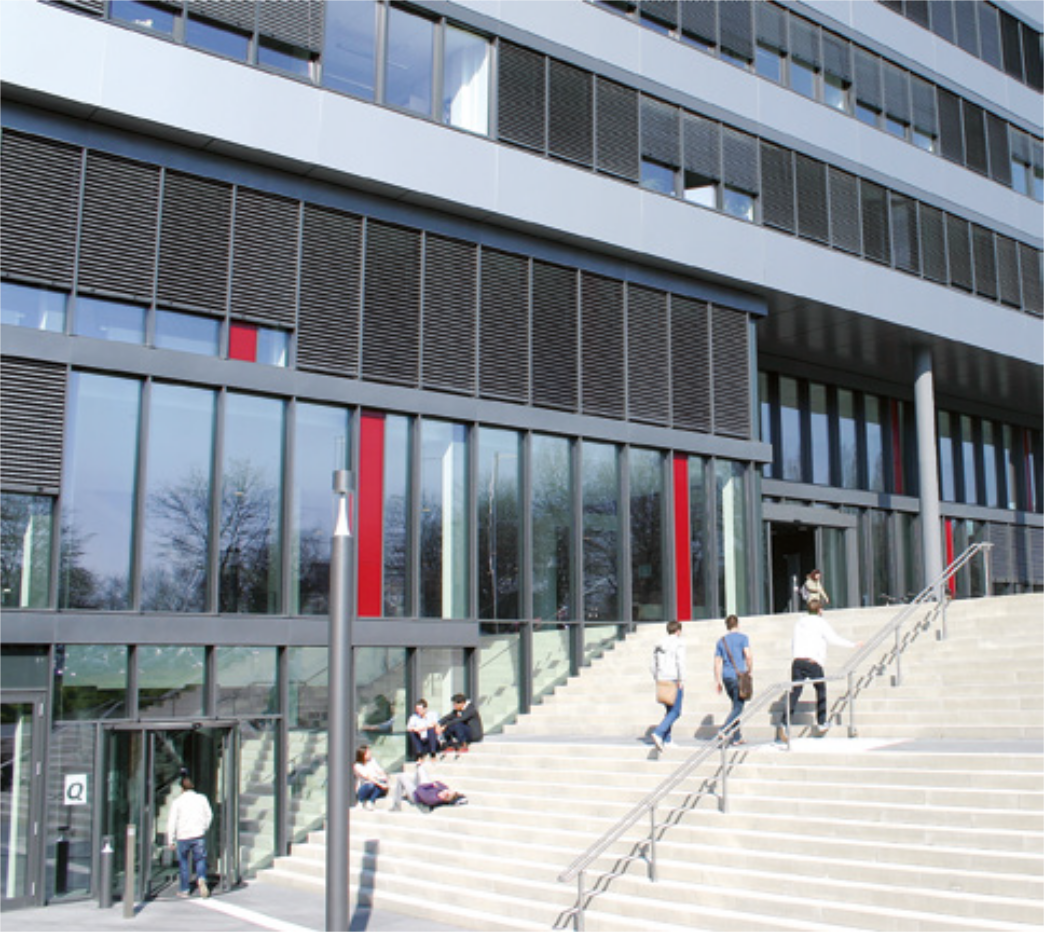
\includegraphics[width=1\textwidth]{\templatePath/images/backgrounds/unibuilding}
		\end{figure}
		
		
	\end{columns}
	
\end{frame}

%------------------------------------------------

\begin{frame}
	\frametitle{Multiple Columns}
	
	\begin{columns}[c]
		
		\column{.33\textwidth}
		\blockheading{Heading}
		
		\begin{itemize}
			\item Statement
			\item Explanation
			\item Example
		\end{itemize}
		
		\column{.33\textwidth}
		\blockheading{Heading}
		
		\begin{itemize}
			\item Statement
			\item Explanation
			\item Example
		\end{itemize}
		
		\column{.33\textwidth}
		\blockheading{Heading}
		
		\begin{itemize}
			\item Statement
			\item Explanation
			\item Example
		\end{itemize}
		
		
	\end{columns}
	
\end{frame}

%%%%%%%%%%%%%%%%%%%%%%%%%%%%%%%%%%%%%%%%%%%%%%%
%%%%%%%%%%%%%%%%%%%%%%%%%%%%%%%%%%%%%%%%%%%%%%%
%%%%%%%%%%%%%%%%%%%%%%%%%%%%%%%%%%%%%%%%%%%%%%%
% Slides end here
%%%%%%%%%%%%%%%%%%%%%%%%%%%%%%%%%%%%%%%%%%%%%%%
%%%%%%%%%%%%%%%%%%%%%%%%%%%%%%%%%%%%%%%%%%%%%%%
%%%%%%%%%%%%%%%%%%%%%%%%%%%%%%%%%%%%%%%%%%%%%%%


%------------------------------------------------

{
	\hnifullbackground 
	
	\begin{frame}
		\textbf{\Huge{\centerline{Thank You!}}}
	\end{frame}
}

\end{document} 

%%%%%%%%%%%%%%%%%%%%%%%%%%%%%%%%%%%%%%%%%%%%%%%
% Author: Ashwin Prasad Shivarpatna Venkatesh 
%%%%%%%%%%%%%%%%%%%%%%%%%%%%%%%%%%%%%%%%%%%%%%%